\papersection{\graphene{} overview}
\label{sec:overview:libos}

\graphene{} is a library OS designed for reusing unmodified applications.
%Existing library OSes have established reuse of single-process applications~\cite{porter11drawbridge}.
The library OSes map a target system API, such as the Linux system calls, to abstractions in \thehostabi{}. %The reduction of host interfaces provides portability to various platforms that can translate the interfaces to host APIs or abstractions,
%and a narrower attack surface that developers can more likely reason about.
% and supporting data structures as library functions---mapping
%high-level APIs onto
%a few paravirtual interfaces to the host kernel.
%Recent library OSes improve efficiency over full guest OSes by eliminating duplicated features
%between the guest and host kernel,
%such as the CPU scheduler, or
%eliminating guest-level multiplexing code, as the library OS supports only one application;
%even compiling out unnecessary guest kernel APIs~\cite{unikernels}.
A library OS is comparable to a partial, guest OS running in a virtual machine.
However, compared with an actual virtual machine, a library OS eliminates duplicated features between the guest to the host kernel, such as the CPU scheduler or file system drivers, and thus reduce the memory footprint of a guest library OS~\cite{porter11drawbridge,unikernels}.
Library OSes have also been proven useful for reusing applications on new hardware platforms, such as \sgx{} enclaves~\cite{baumann14haven}.
%% dp: This sentence seems a little premature
%In recent works, library OSes provide rich OS features for isolated contexts while the host OSes are untrusted

%% Library OSes reduce the memory requirements of running a self-contained,
%% isolated application process
%% %guest \daniela{I would replaced guest by "isolated process or group of processes (a \libos{} instance)''}
%% by orders of magnitude
%% In a cloud computing environment,
%% increasing the number of applications per server has enormous
%% economic benefits.
%% Even on a desktop or portable system, \libos{}es can reduce the overheads
%% of sandboxing untrusted code and running applications
%% designed for another OS.

%Because library OSes execute within a VM \daniela{this phrase does not read good to me because (i) it might imply the picoprocesses need hypervisor support, as misunderstood by reviewer 1 and (ii) you already emphasized the drawbacks of leveraging a VM} or lightweight process ({\em picoprocess}~\cite{xax}),
%library OSes execute with

%% dp: Daniela, great suggestion!  We need to make this situation seem more
%%     like the sky will fall without our help
A key drawback for prior library OSes is the limitation on supporting unmodified, multi-process applications. Many existing applications, such as network servers (e.g., Apache) and shell scripts (e.g., GNU makefiles), create multiple processes for performance scalability, fault isolation, and programmer convenience.
%These applications would benefit from the efficiency and security benefits
%of a library OS.
In order for the efficiency benefits of library OSes to be widely applicable,
especially for unmodified Unix applications,
library OSes must provide commonly-used multi-process abstractions, such as \syscall{fork}, signals, System V IPC message queues and semaphores, sharing file descriptors, and exit notification.
Without sharing memory across processes, the library OS instances must coordinate shared OS states to support multi-process abstractions.
%To support multi-process abstractions, library OSes often have to rely on sharing OS states,
%backed by the hosts' memory sharing features.
For example, \drawbridge{}~\cite{porter11drawbridge} cannot simulate process forking because copy-on-write memory sharing is not a universal OS feature.


\begin{figure}[t!]
\centering
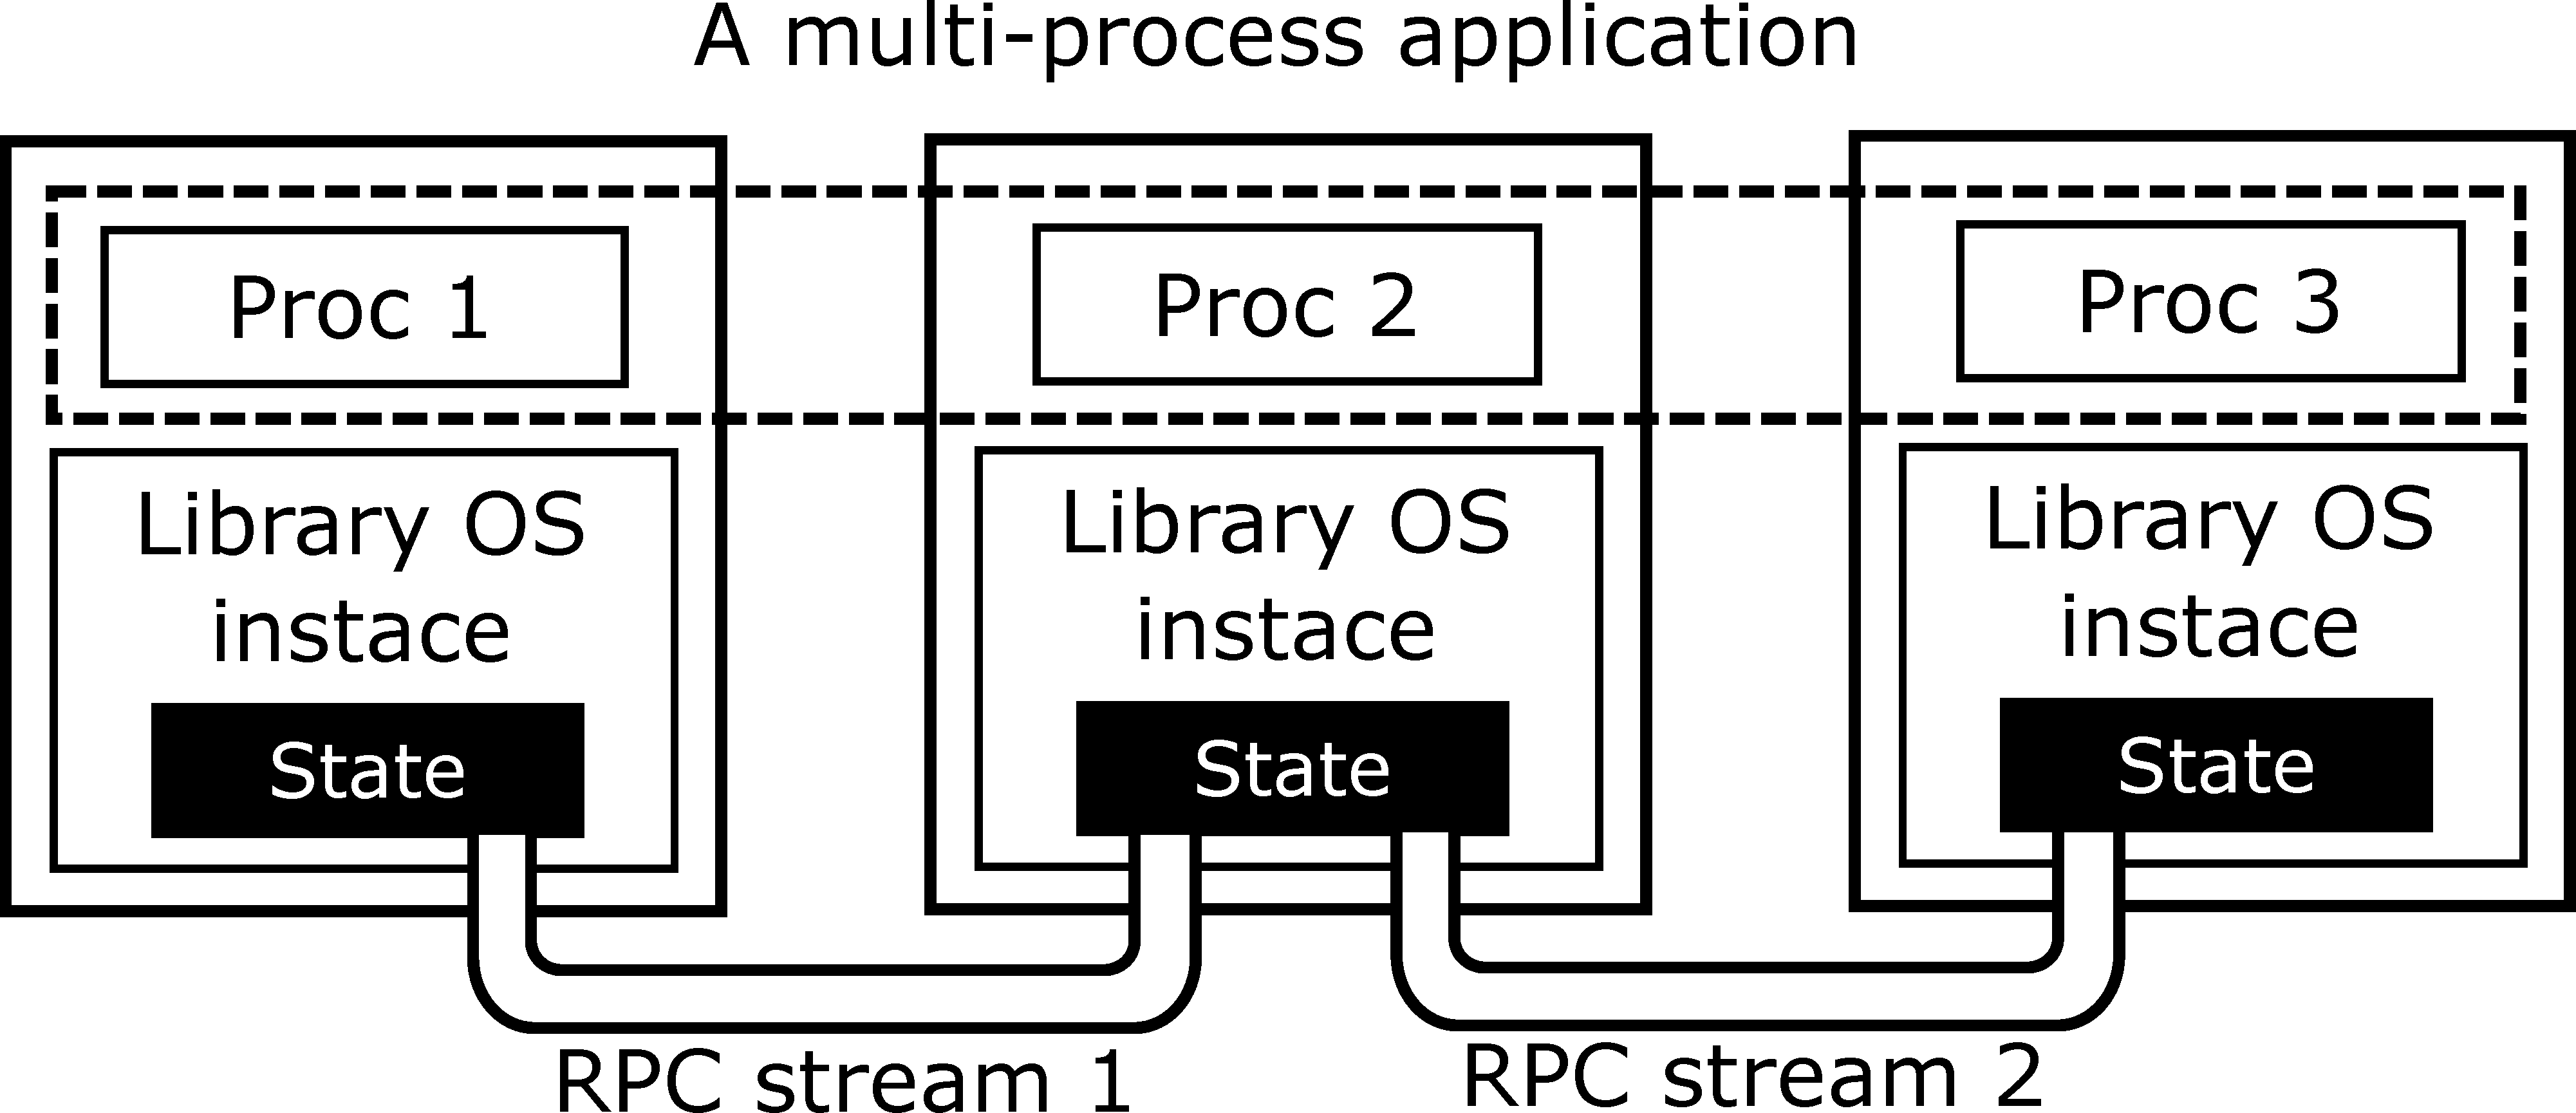
\includegraphics[width=24em]{concept.pdf}
\caption{Multi-process support model of \graphene{} \libos{}. For each process of an application, a \libos{} instance will serve system calls and keep local OS states. States of multi-process abstractions are shared by coordinating over host-provided RPC streams, creating an illusion of running in single OS for the application.}
%\vspace{-.1in}
\label{fig:graphene:concept}
\end{figure}

%{\bf \graphene{}} is a Linux-compatible library OS to run legacy, unmodified Linux applications. 
In \graphene{}, multiple library OS instances collaboratively implement
POSIX abstractions, yet appear to the application as a single, shared OS.
\graphene{} instances coordinate state using RPC streams bridging the processes.
In a distributed POSIX implementation, placement of shared state and messaging complexity are first-order performance concerns.
%We chose to shift implementation complexity into the library OS
%in order to uphold simple enforcement of security isolation in the host.
By coordinating shared states across library OS instances, \graphene{} is able to create an illusion of running in a single OS for multiple processes in an application (Figure~\ref{fig:graphene:concept}).

%Previous library OS designs ensured security isolation of independent applications,
%comparable to a VM, by keeping a relatively narrow host ABI.
%We selected the \graphene{}
%design because it strikes a unique balance between
%and robust, flexible security enforcement.
%The \graphene{} design ensures security isolation of
%mutually distrusting, multi-process
%applications on the same host system.
%Essential to this goal is
%minimally expanding the host ABI to support multi-processing,
%as well as leveraging RPCs as a natural point to mediate inter-\picoproc{} communication.
%RPC coordination among \graphene{} instances can be dynamically disconnected, facilitating novel sandboxing
%techniques.  For instance, we develop an Apache web server extension that, upon logging in a given user,
%places the worker process's \libos{} in a sandbox with access to only that user's data.
%We expect more nuanced degrees of trust are possible in future work.

%\graphene{}'s design gives the user and system administrator a high degree of flexibility
%in isolating arbitrary groups of unmodified application processes,
%while upholding the efficiency and host compatibility benefits of recent library OSes.

%\fixmedp{After a complete draft is written, coalesce all goals and make sure they are addressed early on.  We are doing some scatter-shot motivation}

